\documentclass[english, aspectratio=169]{beamer}
% english is for the language used in standard texts (figures, tables etc)
% aspectratio of 16:9 or set it for more old school to 4:3 (without the ':')

% ---------------------------------------------------------------------------- %
% Load base preamble
% ---------------------------------------------------------------------------- %
\usepackage{import}
\subimport{./preamble/}{beamer.tex}

\usetikzlibrary{fadings}

\usepackage{multirow}

\metroset{sectionpage=none}

% ---------------------------------------------------------------------------- %
% Local settings
% ---------------------------------------------------------------------------- %
% https://tex.stackexchange.com/a/20613
\newcommand\hcancel[2][black]{\setbox0=\hbox{$#2$}%
  \rlap{\raisebox{.35\ht0}{\textcolor{#1}{\rule{\wd0}{1pt}}}}#2}

\newcommand{\B}[0]{\ensuremath{\mathbb{B}}}

\newcommand{\scan}[1]{\text{scan}(#1)}
\newcommand{\sort}[1]{\text{sort}(#1)}

\newcommand{\triple}[3]{\ensuremath{(#1, #2, #3)}}
\renewcommand{\arc}[3]{\ensuremath{#1 \xrightarrow{_{#2}} #3}}

% Horizontal legends: https://tex.stackexchange.com/a/101578
% argument #1: any options
\makeatletter
\newenvironment{customlegend}[1][]{%
    \begingroup
    % inits/clears the lists (which might be populated from previous
    % axes):
    \pgfplots@init@cleared@structures
    \pgfplotsset{#1}%
}{%
    % draws the legend:
    \pgfplots@createlegend
    \endgroup
}%

% makes \addlegendimage available (typically only available within an
% axis environment):
\def\addlegendimage{\pgfplots@addlegendimage}
\makeatother

% difficulty-level in upper right on slides:
\newcommand{\easy}[0]{\faStar[regular]}
\newcommand{\medium}[0]{\faStarHalf*}
\newcommand{\hard}[0]{\faStar[solid]}

% plot styles

\colorlet{adiar}{red}
\colorlet{buddy}{blue!40!purple}

\tikzstyle{plot_adiar}=[color=adiar, mark=diamond*, mark size=2pt, line width=1pt,
                        mark options={color=adiar, fill=adiar, opacity=0.6}]
\tikzstyle{plot_buddy}=[color=buddy, mark=pentagon*, mark size=2pt, line width=1pt,
                        mark options={color=buddy, fill=buddy, opacity=0.6}]

\tikzstyle{dots_buddy}=[color=buddy, mark=pentagon*, mark size=2pt, only marks,
                        mark options={color=buddy, fill=buddy, opacity=0.6}]
\tikzstyle{x_buddy}=[color=buddy, mark=x, mark size=2pt, only marks,
                     mark options={color=buddy, fill=buddy, opacity=0.6}]

% ------------------------------------------------------------------------------
% TITLEPAGE
% ------------------------------------------------------------------------------
\title{Decision Diagrams in External Memory}

\author{Steffan Christ S{\o}lvsten}

\institute{
\includegraphics[width=0.2\linewidth]{external/aulogo_uk_var2_black.eps}}

\date{6\textsuperscript{th} of January 2026}
\begin{document}

% ---------------------------------------------------------------------------- %
\titleframe

\begin{frame}[plain,noframenumbering]{}
  \frametitle{Contents}
  \tableofcontents
\end{frame}

\section{What are Binary Decision Diagrams?}

\begin{frame}[plain,noframenumbering]{}
  \frametitle{Contents}
  \tableofcontents[currentsection]
\end{frame}

\begin{frame}[plain,noframenumbering]{}
  \begin{center}
    {\LARGE\bf Graph-Based Algorithms\\for Boolean Function Manipulation}

    {\large Randal E.\ Bryant}

    {\footnotesize August 1986}
  \end{center}
\end{frame}

\begin{frame}
  \frametitle{\secname}

  % Representation of functions $\B^n \rightarrow \B$ by Bryant '86.

  \begin{figure}
    \centering

    \begin{subfigure}{0.49\linewidth}
      \centering

      \begin{tikzpicture}[scale=1, every node/.style={transform shape}]
        \input{tikz/bdd_example_a.tex}
      \end{tikzpicture}

      \caption{$(x_0 \wedge x_1 \wedge x_3) \vee (x_2 \oplus x_3)$}
    \end{subfigure}
    \begin{subfigure}{0.49\linewidth}
      \centering

      \begin{tikzpicture}[scale=1, every node/.style={transform shape}]
        \input{tikz/bdd_example_b.tex}
      \end{tikzpicture}

      \caption{$\neg(x_0\ ?\ x_2 \wedge x_3 : x_2 \wedge x_3)$}
    \end{subfigure}
  \end{figure}
\end{frame}

\begin{frame}
  \frametitle{\secname}

  \begin{theorem}[Bryant '86]
    For a fixed variable order, if one exhaustively applies the two rules below,
    then one obtains the Reduced OBDD, which is a unique canonical form of the
    function.
  \end{theorem}

  \begin{figure}
    \centering

    \begin{subfigure}[b]{0.40\linewidth}
      \centering

      \begin{tikzpicture}[scale=0.9, every node/.style={transform shape}]
        \input{tikz/reduction_rule_bdd.tex}
      \end{tikzpicture}

      \vspace{10pt}
      {\small {\bf (1)} Remove redundant nodes}
    \end{subfigure}
    \begin{subfigure}[b]{0.59\linewidth}
      \centering

      \begin{tikzpicture}[scale=0.9, every node/.style={transform shape}]
        \input{tikz/reduction_rule_merge.tex}
      \end{tikzpicture}

      \vspace{10pt}
      {\small {\bf (2)} Merge duplicate nodes}
    \end{subfigure}

  \end{figure}
\end{frame}

\begin{frame}
  \frametitle{\secname}

  Let $N_f$, $N_g$ be the size of the BDDs for $f$ and $g$ and let $T$ be the $O(N_f \cdot N_g)$
  size of the BDD for $f \odot g$.

  \begin{theorem}
    \lstinline{bdd_apply(f,g,}$\odot$\lstinline{)} runs in $O(N_f + N_g + T)$
    time
  \end{theorem}
  \begin{itemize}
  \item Memoisation (\emph{Computation Cache}) ensures each $(t_f,t_g)$ is
    only computed once.

  \item Reduction Rules can be maintained with a
    \texttt{make\_node($i$,$t$,$e$)} in $O(1)$ time.
    \begin{enumerate}
    \item Redundancy is resolved with an if-statement.
    \item Duplication is avoided with a hash table (\emph{Unique Node Table}).
    \end{enumerate}
  \end{itemize}

  \begin{corollary}
    \lstinline{bdd_apply(f,g,}$\odot$\lstinline{)} runs in $O(1)$ time per BDD node.
  \end{corollary}
\end{frame}

\begin{frame}
  \frametitle{\secname}

  \begin{figure}
    \centering

    \begin{tikzpicture}
      \begin{axis}[%
        width=0.69\linewidth, height=0.42\linewidth,
        every tick label/.append style={font=\scriptsize},
        % x-axis
        xlabel={Number of BDD Nodes},
        xmajorgrids=true,
        xmin=800000 ,
        xmax=1200000000,
        xmode = log,
        % y-axis
        ymin=0.1,
        ymax=0.27,
        ylabel={$\mu$s / BDD Node},
        ytick distance={0.05},
        yminorgrids=false,
        ymajorgrids=true,
        grid style={dashed,black!20},
        ]

        \addplot [style=plot_buddy]
        table {./data/cache_buddy_time_per_node.tex};
      \end{axis}
    \end{tikzpicture}

    \caption{Running time of \emph{BuDDy} for the $N$-Queens problem.}
  \end{figure}
\end{frame}

\begin{frame}
  \frametitle{\secname}

  \begin{figure}
    \centering

    \begin{tikzpicture}
      \begin{axis}[%
        width=0.69\linewidth, height=0.42\linewidth,
        every tick label/.append style={font=\scriptsize},
        % x-axis
        xlabel={Memory (GiB)},
        xmajorgrids=true,
        xmin=3.5,
        xmax=10.5,
        xtick={4, ..., 10},
        % y-axis
        ylabel={time (seconds)},
        yminorgrids=false,
        ymajorgrids=true,
        grid style={dashed,black!20},
        ]

        \draw [white, pattern=north west lines, pattern color=black!30!white]
        (axis cs: 8, 0) rectangle (axis cs: 10, 3000);

        \addplot[thick, samples=1, smooth, black, name path=barrier]
        coordinates {(8,0)(8,3000)};

        \node[black] at (axis cs: 7.6, 2800){\tiny{RAM}};
        \node[black] at (axis cs: 8.4, 2800){\tiny{Swap}};

        \addplot [style=plot_buddy]
        table {./data/cache_buddy_swap.tex};
      \end{axis}
    \end{tikzpicture}

    \caption{Running time of \emph{BuDDy} for \emph{3D Tic-Tac-Toe} with $N=21$.}
  \end{figure}
\end{frame}

\section{Why do they break?}

\begin{frame}[plain,noframenumbering]{}
  \frametitle{Contents}
  \tableofcontents[currentsection]
\end{frame}

\begin{frame}
  \frametitle{\secname}

  \input{anim/io_model__motivation.tex}
\end{frame}

\begin{frame}
  \frametitle{\secname}

  \begin{figure}
    \centering

    \input{tikz/io_model.tex}

    \caption{The I/O model by Aggarwal and Vitter '87}
  \end{figure}
\end{frame}

\section{How can we fix it?}

\begin{frame}[plain,noframenumbering]{}
  \frametitle{Contents}
  \tableofcontents[currentsection]
\end{frame}

\begin{frame}[plain,noframenumbering]{}
  \begin{center}
    {\LARGE\bf The I/O-Complexity of Ordered\\Binary-Decision Diagram Manipulation}

    Lars Arge

    % {\footnotesize Department of Computer Science\\University of Aarhus}

    {\footnotesize August 1996}
  \end{center}
\end{frame}

\subsection{Time-forward Processing}

\begin{frame}
  \frametitle{\secname}

  \begin{columns}
    \begin{column}{0.6\textwidth}
      \Large

      Processing Order
      \begin{itemize}
      \item<1-> \textbf{Depth-first}:\\
        \emph{Last in, first out} Queue (Stack)
      \item<9-> \textbf{Breadth-first}:\\
        \emph{First in, first out} Queue
      \item<17-> \textbf{Time-forward Processing}:\\
        \emph{Priority} Queue
      \end{itemize}
    \end{column}
    \begin{column}{0.4\textwidth}
      \centering

      \resizebox{0.7\textwidth}{!}{%
        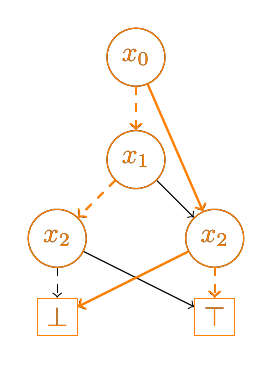
\begin{tikzpicture}
          % Fig 1.4 but with x0, x1, and x2
\node[shape=circle, draw=black, fill=white] at (0, 0.3)
(r) {$x_0$};

\node[shape=circle, draw=black, fill=white] at ( 0, -1)
(y) {$x_1$};

\node[shape=circle, draw=black, fill=white] at (-1, -2)
(g1) {$x_2$};

\node[shape=circle, draw=black, fill=white] at ( 1, -2)
(g2) {$x_2$};

\node[shape=rectangle, draw=black, fill=white] at (-1,-3)
(bot) {$\bot$};
\node[shape=rectangle, draw=black, fill=white] at ( 1,-3)
(top) {$\top$};

\draw[->, dashed]
  (r)  edge (y)
  (y)  edge (g1)
  (g1) edge (bot)
  (g2) edge (top)
;
\draw[->]
  (r)  edge (g2)
  (y)  edge (g2)
  (g1) edge (top)
  (g2) edge (bot)
;


          % nodes
          \onslide<2,10> {
            \node[orange, shape=circle, draw=orange] at (0, 0.3)
            {$x_0$};
          }
          \onslide<6,12> {
            \node[orange, shape=circle, draw=orange] at ( 0, -1)
            {$x_1$};
          }
          \onslide<7,15> {
            \node[orange, shape=circle, draw=orange] at (-1, -2)
            {$x_2$};
          }
          \onslide<3,11> {
            \node[orange, shape=circle, draw=orange] at ( 1, -2)
            {$x_2$};
          }
          \onslide<4,13> {
            \node[orange, shape=rectangle, draw=orange] at (-1,-3)
            {$\bot$};
          }
          \onslide<5,14> {
            \node[orange, shape=rectangle, draw=orange] at ( 1,-3)
            {$\top$};
          }

          % edges
          \onslide<3-8,11-16> {
            \draw[->, orange, thick] (r) edge (g2);
          }
          \onslide<6-8,12-16> {
            \draw[->, dashed, orange, thick] (r) edge (y);
          }
          \onslide<7-8,15-16> {
            \draw[->, dashed, orange, thick] (y) edge (g1);
          }
          \onslide<4-8,13-16> {
            \draw[->, orange, thick] (g2) edge (bot);
          }
          \onslide<5-8,14-16> {
            \draw[->, dashed, orange, thick] (g2) edge (top);
          }
        \end{tikzpicture}
      }
    \end{column}
  \end{columns}
\end{frame}

\begin{frame}
  \frametitle{\subsecname}

  \begin{columns}
    \begin{column}{0.27\textwidth}
      \centering

      \resizebox{\textwidth}{!}{%
        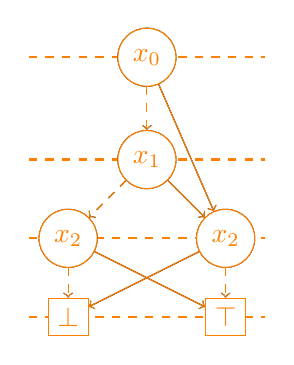
\begin{tikzpicture}
          \onslide<2>   { \draw[orange, thick, dashed] (-1.5, 0.3) -- ++(3, 0); }
          \onslide<3>   { \draw[orange, thick, dashed] (-1.5,-1)   -- ++(3, 0); }
          \onslide<4-5> { \draw[orange, thick, dashed] (-1.5,-2)   -- ++(3, 0); }
          \onslide<6-7> { \draw[orange, thick, dashed] (-1.5,-3)   -- ++(3, 0); }

          % Nodes
          % Fig 1.4 but with x0, x1, and x2
\node[shape=circle, draw=black, fill=white] at (0, 0.3)
(r) {$x_0$};

\node[shape=circle, draw=black, fill=white] at ( 0, -1)
(y) {$x_1$};

\node[shape=circle, draw=black, fill=white] at (-1, -2)
(g1) {$x_2$};

\node[shape=circle, draw=black, fill=white] at ( 1, -2)
(g2) {$x_2$};

\node[shape=rectangle, draw=black, fill=white] at (-1,-3)
(bot) {$\bot$};
\node[shape=rectangle, draw=black, fill=white] at ( 1,-3)
(top) {$\top$};

\draw[->, dashed]
  (r)  edge (y)
  (y)  edge (g1)
  (g1) edge (bot)
  (g2) edge (top)
;
\draw[->]
  (r)  edge (g2)
  (y)  edge (g2)
  (g1) edge (top)
  (g2) edge (bot)
;


          % Node Highlights
          \onslide<2> {
            \node[orange, shape=circle, draw=orange, fill=white] at (0, 0.3)
            (r) {$x_0$};

            \draw[orange, ->, dashed] (r) edge (y);
            \draw[orange, ->]         (r) edge (g2);
          }
          \onslide<3> {
            \node[orange, shape=circle, draw=orange, fill=white] at ( 0, -1)
            (y) {$x_1$};

            \draw[orange, ->, dashed] (y) edge (g1);
            \draw[orange, ->]         (y) edge (g2);
          }
          \onslide<4> {
            \node[orange, shape=circle, draw=orange, fill=white] at (-1, -2)
            (g1) {$x_2$};

            \draw[orange, ->, dashed] (g1) edge (bot);
            \draw[orange, ->]         (g1) edge (top);
          }
          \onslide<5> {
            \node[orange, shape=circle, draw=orange, fill=white] at ( 1, -2)
            (g2) {$x_2$};

            \draw[orange, ->, dashed] (g2) edge (top);
            \draw[orange, ->]         (g2) edge (bot);
          }
          \onslide<6> {
            \node[orange, shape=rectangle, draw=orange, fill=white] at (-1,-3)
            (bot) {$\bot$};
          }
          \onslide<7> {
            \node[orange, shape=rectangle, draw=orange, fill=white] at ( 1,-3)
            (top) {$\top$};
          }
        \end{tikzpicture}
      }
    \end{column}
    \begin{column}{3em}
      $\implies$
    \end{column}
    \begin{column}{0.53\textwidth}
      \centering

      \only<1-7>{\resizebox{\textwidth}{!}{%
        \begin{tikzpicture}
          \node[shape=circle, draw=black] at (0, 0)
          (r) {$x_0$};

          \node[shape=circle, draw=black] at (1, 0)
          (y) {$x_1$};

          \node[shape=circle, draw=black] at (2, 0)
          (g1) {$x_2$};

          \node[shape=circle, draw=black] at (3, 0)
          (g2) {$x_2$};

          \node[shape=rectangle, draw=black] at (4,0)
          (bot) {$\bot$};
          \node[shape=rectangle, draw=black] at (5,0)
          (top) {$\top$};

          \draw[->, dashed]
            (r)  edge (y)
            (y)  edge (g1)
            (g1) edge[bend right=40] (bot)
            (g2) edge[bend left=40]  (top)
          ;
          \draw[->]
            (r)  edge[bend left=40] (g2)
            (y)  edge[bend left=40] (g2)
            (g1) edge[bend right=45] (top)
            (g2) edge (bot)
          ;

          \only<2> {
            \node[orange, shape=circle, draw=orange] at (0, 0)
            (r) {$x_0$};

            \draw[orange, ->, dashed] (r) edge (y);
            \draw[orange, ->]         (r) edge[bend left=40] (g2);
          }
          \only<3> {
            \node[orange, shape=circle, draw=orange] at (1, 0)
            (y) {$x_1$};

            \draw[orange, ->, dashed] (y) edge (g1);
            \draw[orange, ->]         (y) edge[bend left=40] (g2);
          }
          \only<4> {
            \node[orange, shape=circle, draw=orange] at (2, 0)
            (g1) {$x_2$};

            \draw[orange, ->, dashed] (g1) edge[bend right=40] (bot);
            \draw[orange, ->]         (g1) edge[bend right=45] (top);
          }
          \only<5> {
            \node[orange, shape=circle, draw=orange] at (3, 0)
            (g2) {$x_2$};

            \draw[orange, ->, dashed] (g2) edge[bend left=40]  (top);
            \draw[orange, ->]         (g2) edge (bot);
          }
          \only<6> {
            \node[orange, shape=rectangle, draw=orange] at (4,0)
            (bot) {$\bot$};
          }
          \only<7> {
            \node[orange, shape=rectangle, draw=orange] at (5,0)
            (top) {$\top$};
          }
        \end{tikzpicture}
      }}
    \only<8->{
      { \LARGE
        \begin{tabular}{r c l}
          [ & $\triple{(0,0)}{(1,0)}{(2,0)}$ & ,
          \\
            & $\triple{(1,0)}{(2,0)}{(2,1)}$ & ,
          \\
            & $\triple{(2,0)}{\top}{\bot}$   & ,
          \\
            & $\triple{(2,1)}{\bot}{\top}$   & ]
        \end{tabular}
      }
    }
    \end{column}
  \end{columns}
\end{frame}

\begin{frame}[t]
  \frametitle{\subsecname\quad \emph{CountPaths Example}}

  \begin{figure}
    \centering

    \begin{tikzpicture}[scale=0.9, every node/.style={transform shape}]
      \input{tikz/count_paths__idea.tex}
    \end{tikzpicture}
  \end{figure}

  \only<1>{
    \begin{center}
      {\Large \textbf{Idea}}

      {\large Count the number of in-going paths to each node.}
    \end{center}
  }

  \only<2->{
    \begin{center}
      {\Large \textbf{Time-Forward Processing}}

      Defer work with $Q_{\mathit{count}}$ : \texttt{PriorityQueue}$\langle (\arc{s}{}{t}, \quad
      \N) \rangle$ sorted on $t$ in ascending order.

      $(\arc{(i,\texttt{id})}{\bot}{\alpha}, \quad \sum_i n_i)$, \qquad
      $(\arc{(i,\texttt{id})}{\top}{\beta}, \quad \sum_i n_i)$
    \end{center}
  }
\end{frame}

\begin{frame}
  \frametitle{\subsecname\quad \emph{CountPaths Example}}

  \input{anim/count_paths_tfp.tex}
\end{frame}

\blankframe

\subsection{Adiar}

\input{fram/adiar.tex}

\begin{frame}[t]
  \begin{center}
    \Large
    Quantified Boolean Formul{\ae} (QBF) of 2-player games:\\
    {$\exists \vec{x} \forall \vec{y} \dots \exists \vec{z} : \phi(\vec{x}, \vec{y}, \dots, \vec{z}) \stackrel{?}{=} 1$}
  \end{center}

  \begin{center}
    \begin{tikzpicture}
      \begin{axis}[%
        width=0.8\linewidth, height=0.42\linewidth,
        every tick label/.append style={font=\scriptsize},
        % x-axis
        xlabel={\small \texttt{Adiar} Running Time (s)},
        xmin=0.01,
        xmax=10000,
        xtick={0.01,0.1,1,10,100,1000,10000},
        xmode=log,
        % y-axis
        ylabel={\small \texttt{BuDDy} Relative Running Time},
        ymin=0.00390625,
        ymax=5.0,
        ytick = {0.00390625,0.015625,0.0625,0.25,1,4},
        yticklabels = {
          $2^{-8} \times$,
          $2^{-6} \times$,
          $2^{-4} \times$,
          $2^{-2} \times$,
          $1 \times$,
          $2^{2} \times$
        },
        ymode=log,
        % grid
        grid style={dashed,black!12},
        ]

        % 1 line
        \addplot[domain=0.001:100000, samples=8, color=black]
        {1};

        % vertical 1s line
        \draw[densely dotted, opacity=0.4] (0,1.0) -- (0,-5.0);
        % vertical 100s line
        \draw[densely dotted, opacity=0.4] (4.6,1.0) -- (4.6,-5.0);

        % data (solved)
        \addplot+ [forget plot, style=dots_buddy, mark size=5pt]
        table {./data/qbf.buddy.solved.tex};

        % data (timeouts)
        \addplot+ [forget plot, style=x_buddy, mark size=4pt]
        table {./data/qbf.buddy.timeouts.tex};
      \end{axis}
    \end{tikzpicture}
  \end{center}
\end{frame}

\begin{frame}[t]
  \begin{center}
    \Large
    Relational Product in a Transition System:\\
    $\mathit{RelProd}(S_{\vec{x}}, T_{\vec{x}, \vec{x}'}) \triangleq
    (\exists \vec{x}\ .\ S_{\vec{x}} \land T_{\vec{x}, \vec{x}'})[\vec{x}' \mapsto \vec{x}]$
  \end{center}

  \begin{figure}
    \centering

    \begin{subfigure}{0.3\linewidth}
      \centering

      \qquad\quad{\tiny \texttt{GPUForwardProgress}~20a}

      \begin{tikzpicture}
        \begin{axis}[%
          width=1.05\linewidth, height=1\linewidth,
          every tick label/.append style={font=\scriptsize},
          % x-axis
          xlabel={\scriptsize Memory (GiB)},
          xmin=0.8,
          xtick={1,2,4,8},
          xticklabels={1,2,4,8},
          xmax=10,
          xmode=log,
          % y-axis
          ylabel={\scriptsize Running Time (s)},
          ymin=100,
          ymax=43200,
          ytick={100,1000,10000,100000},
          ymode=log,
          % grid
          grid style={dashed,black!12},
          ]

          % BuDDy memory out
          % \addplot+ [style=x_buddy, forget plot] coordinates {
          % (2, 36000)
          % };

          %   data
          \addplot+ [style=plot_adiar]
          table {./data/memory.gpufp_20_a.adiar.tex};

          \addplot+ [style=plot_buddy]
          table {./data/memory.gpufp_20_a.buddy.tex};
        \end{axis}
      \end{tikzpicture}

    \end{subfigure}
    \hspace{-30pt}
    \begin{subfigure}{0.3\linewidth}
      \centering

      \quad{\tiny \texttt{SmartHome}~16}

      \begin{tikzpicture}
        \begin{axis}[%
          width=1.05\linewidth, height=1\linewidth,
          every tick label/.append style={font=\scriptsize},
          % x-axis
          xlabel={\scriptsize Memory (GiB)},
          xmin=0.8,
          xtick={1,2,4,8},
          xticklabels={1,2,4,8},
          xmax=10,
          xmode=log,
          % y-axis
          ymin=100,
          ymax=43200,
          ytick={100,1000,10000,100000},
          yticklabels={,,,},
          ymode=log,
          % grid
          grid style={dashed,black!12},
          ]

          % BuDDy memory out
          % \addplot+ [style=x_buddy, forget plot] coordinates {
          % (2, 36000)
          % };

          %   data
          \addplot+ [style=plot_adiar]
          table {./data/memory.smhome_16.adiar.tex};

          \addplot+ [style=plot_buddy]
          table {./data/memory.smhome_16.buddy.tex};
        \end{axis}
      \end{tikzpicture}
    \end{subfigure}
    \hspace{-36.8pt}
    \begin{subfigure}{0.5\linewidth}
      \centering

      \quad{\tiny \texttt{ShieldPPPs}~10a}

      \begin{tikzpicture}
        \begin{axis}[%
          width=1.1\linewidth, height=0.6\linewidth,
          every tick label/.append style={font=\scriptsize},
          % x-axis
          xlabel={\scriptsize Memory (GiB)},
          xmin=0.8,
          xtick={1,2,4,8,16,32,64},
          xticklabels={1,2,4,8,16,32,64},
          xmax=80,
          xmode=log,
          % y-axis
          ymin=100,
          ymax=43200,
          ytick={100,1000,10000,100000},
          yticklabels={,,,},
          ymode=log,
          % grid
          grid style={dashed,black!12},
          ]

          % BuDDy time out
          \addplot+ [style=x_buddy, forget plot] coordinates {
            (2, 36000)
            (4, 36000)
            (8, 36000)
          };

          % data
          \addplot+ [style=plot_adiar]
          table {./data/memory.shield_s_ppp_010_a.adiar.tex};

          \addplot+ [style=plot_buddy]
          table {./data/memory.shield_s_ppp_010_a.buddy.tex};
        \end{axis}
      \end{tikzpicture}
    \end{subfigure}

    \smallskip

    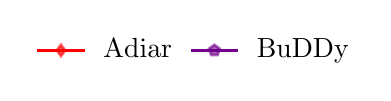
\begin{tikzpicture}
      \begin{customlegend}[
        legend columns=-1,
        legend style={draw=none,column sep=1ex},
        legend entries={
          Adiar,
          BuDDy
        }
        ]
        \addlegendimage{style=plot_adiar}
        \addlegendimage{style=plot_buddy}
      \end{customlegend}
    \end{tikzpicture}

    %\caption{Relational Product for MCC models with a $2^{25}$ state space BDD. Timeouts are marked
    %         as stars.}
  \end{figure}
\end{frame}

\section{What's next?}

\begin{frame}[plain,noframenumbering]{}
  \frametitle{Contents}
  \tableofcontents[currentsection]
\end{frame}

\begin{frame}
  \frametitle{\secname}

  \begin{center}
    \begin{tikzpicture}
      \input{tikz/timeline.tex}
    \end{tikzpicture}
  \end{center}
\end{frame}

\begin{frame}
  \frametitle{\secname\quad \emph{Node Table}}

  \textbf{Problem}\\
  \emph{Adiar runs very slow on small instances!}

  \textbf{Observation (S{\o}lvsten~'25)}\\
  \emph{Adiar's algorithms can use the conventional node table as its input and/or output.}

  \pause
  \smallskip
  \textbf{Solution (S{\o}lvsten~'25)}\\
  \begin{itemize}
  \item \emph{Implement a node table\footnote{The design of the node table in the setting of Adiar
        has its own novel research opportunities.} in Adiar.}
  \item \emph{Use recursion until the BDDs get too large. Use time-forward processing to migrate to
      disk (for free!) and compute the next BDD.}
  \item \emph{When the BDD becomes small, output (for free!) back into the table and continue with
      recursion.}
  \end{itemize}
\end{frame}

\begin{frame}
  \frametitle{\secname\quad \emph{Variable Ordering}}

  \begin{theorem}[S{\o}lvsten~'25]
    The time and I/O complexity of \texttt{bdd\_replace($f$, $\pi$)} is
    $\Oh{\sort{T \cdot \sum_{i=1}^n C^{\emptyset}_{1:f[i]}}}$.
  \end{theorem}
  Hence, we can create an I/O-efficient variants of \emph{Simulated Annealing},
  \emph{Genetic Algorithms}, \emph{Ant Colony Simulation}, and more.

  \pause
  \begin{theorem}[S{\o}lvsten~'25]
    If $\pi$ only swaps two variables, then time and I/O complexity is
    $\Oh{\sort{N+T}}$.
  \end{theorem}
  Hence, we can recreate \emph{Rudell's Sifting} algorithm.

  \pause
  \begin{theorem}[S{\o}lvsten~'25]
    If $\pi$ only swaps adjacent variables, then time and I/O complexity is
    $\Oh{\sort{N+T}}$.
  \end{theorem}
  Hence, we can recreate the \emph{2-Window} algorithm.

\end{frame}

\begin{frame}
  \frametitle{\secname\quad \emph{Other Decision Diagrams}}

  \begin{columns}
    \begin{column}[t]{0.49\linewidth}

      \begin{itemize}
      \item[\faIcon{check-circle}] Binary Decision Diagrams

        [TACAS '22]
      \item[\faIcon{check-circle}] Zero-suppressed BDDs

        [NFM '23]
        \begin{itemize}
        \item \emph{Policy} pattern
        \end{itemize}
      \item[\faIcon{circle}] BDDs with Complemented Edges
        \begin{itemize}
        \item Mark bit on unique identifier (\texttt{uid}).
        \item Extend \texttt{Reduce} for normalization.
        \end{itemize}
      \end{itemize}

    \end{column}
    \begin{column}[t]{0.49\linewidth}

      \begin{itemize}
      \item[\faIcon{circle}] Multi-terminal BDDs
        \begin{itemize}
        \item Add non-binary terminals in \texttt{uid}.
        \item Generalize \emph{i-level cuts} for non-binary terminals.
        \item Add \texttt{mtbdd} policy.
        \end{itemize}
      \item[\faIcon{circle}] Edge-valued BDDs
        \begin{itemize}
        \item Add \emph{weight} on edges.
        \item Extend \texttt{Reduce} for normalization.
        \item Add \texttt{evdd} policy.
        \end{itemize}
      \end{itemize}

    \end{column}
  \end{columns}
\end{frame}

\blankframe

\input{fram/endslate.tex}

\end{document}
